\documentclass[11pt,a4paper]{article}

\usepackage{style2017}
\usepackage{hyperref}

\hypersetup{
    colorlinks =false,
    linkcolor=blue,
   linkbordercolor = 1 0 0
}
\newcounter{numexo}
\setcellgapes{1pt}

\begin{document}



\begin{NSI}
{Exercice}{Listes}
\end{NSI}


\addtocounter{numexo}{1}
\subsection*{\Large Exercice \thenumexo}
La suite de Fibonacci est une suite dont chaque valeur s'obtient en ajoutant les deux valeurs qui la précèdent, avec les nombres $0$ et $1$ comme valeurs initiales.

Soit \textbf{t} la liste des premiers nombres de la suite de Fibonacci: $$t=[0,1,1,2,3,5,8,13,21,34,55,89]$$
\begin{enumerate}
\item Saisir la liste \textbf{t} donnée ci-dessus.
\item Afficher sur 3 lignes, avec une seule instruction \textbf{print}, la longueur de ce tableau, le premier élément et son dernier élément. Vous devez obtenir :

\begin{center}
\fbox{\begin{minipage}{8cm}
nombre de valeurs : 12 \\
premier élément : 0 \\
dernier élément : 89
\end{minipage}
}
\end{center}
\item \begin{enumerate}
\item Créer un second tableau t1 de la même dimension que t dont toutes valeurs sont 0.
\item En utilisant une boucle \textbf{for}, compléter le tableau t1 avec les valeurs du tableau t rangées dans l'ordre inverse. On doit obtenir :

\begin{center}
\fbox{\begin{minipage}{8cm}
[89,55,34,21,13,8,5,3,2,1,1,0]
\end{minipage}
}
\end{center}
\end{enumerate} 
\item Créer un tableau dont les valeurs sont la somme des valeurs des tableaux t et t1 de même indice.
\item Créer la fonction \textbf{terme\_suivant} qui prend en paramètre la liste des nombres de la suite de Fibonacci et ajoute le terme suivant en fin de liste.
\end{enumerate}

\addtocounter{numexo}{1}
\subsection*{\Large Exercice \thenumexo}
\begin{enumerate}
\item Créer une fonction \textbf{tabalea} qui renvoie un tableau avec des entiers choisis aléatoirement compris entre 1 et 100 et dont la dimension sera passée en paramètre. 

\textit{Par exemple :} \textbf{tabalea}(50) renvoie un tableau avec 50 entiers aléatoirement pris entre 1 et 100.
\item Créer une fonction \textbf{tabmax} qui prend en paramètre un tableau et qui renvoie son plus grand élément et son indice.
\item Créer une fonction \textbf{tabin} qui prend en paramètres un nombre entier et un tableau et renvoie \textbf{True} si le nombre est présent dans le tableau et \textbf{False} dans le cas contraire.
\item Créer une fonction \textbf{tabmode} qui prend en paramètre un tableau et renvoie la valeur dominante, c'est à dire la valeur du tableau la plus représentée, et le nombre de fois que celle-ci est présente.
\item Créer la fonction \textbf{permute} qui prend en paramètre la liste de nombres et la modifie en décalant toutes les valeurs de 1 rang vers la droite. La première position, laissée libre, sera occupée par la dernière valeur du tableau qui a été éjectée.  
\end{enumerate}


\addtocounter{numexo}{1}
\subsection*{\Large Exercice \thenumexo }
\begin{enumerate}
\item Créer un tableau de 8 valeurs, chaque valeur étant un fruit commençant par une lettre différente ! Trier le tableau avec la fonction sort.
\item Créer une fonction \textbf{échange} prenant en paramètre un tableau et deux indices i et j et qui renvoie le tableau avec les valeurs d'indices i et j permutées.
\item Créer une fonction \textbf{mélange} qui prend en paramètre un tableau et mélange aléatoirement les valeurs de ce tableau. On pourra utiliser la fonction échange à plusieurs reprises avec des indices choisis aléatoirement.
\end{enumerate}


\addtocounter{numexo}{1}
\subsection*{\Large Exercice \thenumexo }
Créer les tableaux suivants avec la méthode par compréhension:
\begin{enumerate}
\item Liste des nombres entiers de 0 à 12 inclus
\item Liste des nombres entiers pairs de 0 à 16 inclus
\item Liste des nombres impairs de 1 à 15 inclus
\item Liste des carrés des nombres entiers de 1 à 5 inclus
\item Liste des lettres de l'alphabet en majuscule
\item $[[0, 0, 0, 0], [0, 0, 0, 0], [0, 0, 0, 0], [0, 0, 0, 0]]$
\item $[[1, 2, 3, 4], [5, 6, 7, 8], [9, 10, 11, 12], [13, 14, 15, 16]]$
\end{enumerate}


\addtocounter{numexo}{1}
\subsection*{\Large Exercice \thenumexo }
\begin{enumerate}
\item Créer un tableau t de dimension aléatoire n dont les valeurs sont des nombres entiers consécutifs inférieurs à 20. Par exemple, si n=4, alors t=[0,1,2,3,4]
\item Créer une fonction \textbf{prolonge} qui ajoute au tableau t de nombres entiers rangés par ordre croissant, le nombres entiers consécutifs jusqu'à 20.
\item Créer une fonction \textbf{miroir} qui ajoute au tableau t de nombres entiers rangés par ordre croissant, les nombres entiers décroissants jusqu'à 0 sans aucune répétition.
\end{enumerate}


\addtocounter{numexo}{1}
\subsection*{\Large Exercice \thenumexo }
\begin{enumerate}
\item Créer deux tableaux \textbf{jours} et \textbf{mois} regroupant toutes les valeurs possibles.
\item Créer la fonction \textbf{affiche\_janvier} affichant tout le mois de janvier commençant par un lundi 1 janvier.
\item Modifier la fonction \textbf{affiche\_janvier} prenant en paramètre le premier jour du mois (lundi, mardi, mercredi,...) et affichant le mois en conséquence.
\item Créer la fonction \textbf{affiche\_mois} prenant comme paramètre un mois et le premier jour du mois et affichant le mois. On prendra en compte le nombre de jours dans le mois.
\item Écrire une fonction \textbf{est\_bissextile} prenant en paramètre l'année et retourne \textbf{True} si elle est bissextile ou \textbf{False} dans le cas contraire. On rappelle qu'une année est bissextile si elle est un multiple de 4 mais pas un multiple de 100, ou si elle est un multiple de 400.
\item Modifier la fonction \textbf{affiche\_mois} en ajoutant comme paramètre l'année et affichant le mois de février avec 28 ou 29 jours.
\item Modifier la fonction \textbf{affiche\_mois} pour qu'elle retourne un tableau des dates demandées.
\end{enumerate}



\addtocounter{numexo}{1}
\subsection*{\Large Exercice \thenumexo }
\begin{enumerate}
\item Créer une fonction \textbf{nouvelleGrille} qui crée un tableau de tableaux de dimension $10 \times 10$, c'est à dire de $10$ lignes et $10$ colonnes initialisée avec des zéros.\\
Créer la variable \textbf{maGrille} qui est une grille $10 \times 10$ de zéros.
\item Créer une fonction \textbf{alimente} qui remplit la grille avec des nombres entiers aléatoirement choisis entre 0 et 200. Alimenter la variable ma\_grille.
\item Créer une fonction \textbf{tabmax} qui renvoie la plus grande valeur d'un tableau (voir exercice 2).
\item Créer une fonction \textbf{transpose} qui prend en paramètre une grille et renvoie une grille dont les lignes sont les colonnes de la grille saisie en paramètre.
\item Créer une fonction \textbf{maxiligne} qui renvoie un tableau contenant la valeur maximale de chaque ligne de la grille. Penser à utiliser la fonction tabmax.
\item Créer une fonction \textbf{maxicolonne} qui renvoie un tableau contenant la valeur maximale de chaque colonne de la grille. Penser à utiliser la fonction tabmax et la fonction transpose.
\end{enumerate}

\newpage
\addtocounter{numexo}{1}
\subsection*{\Large Exercice \thenumexo }
Le Verger est un jeu de société coopératif créé en 1986. Ce jeu contient:
\begin{itemize}
\item un plan de jeu présentant 4 arbres fruitiers (prunier, pommier, poirier, cerisier) ainsi qu'un corbeau au centre.
\item 40 fruits (10 pour chaque arbre du plan de jeu) en bois à disposer sur chacun des arbres.
\item 4 paniers pour les joueurs (1 panier par joueur)
\item Un puzzle corbeau de 9 pièces que l'on reconstitue lors de la partie.
\item Un dé dont les faces représentent les 4 arbres, le panier et le corbeau.
\end{itemize}

\begin{center}
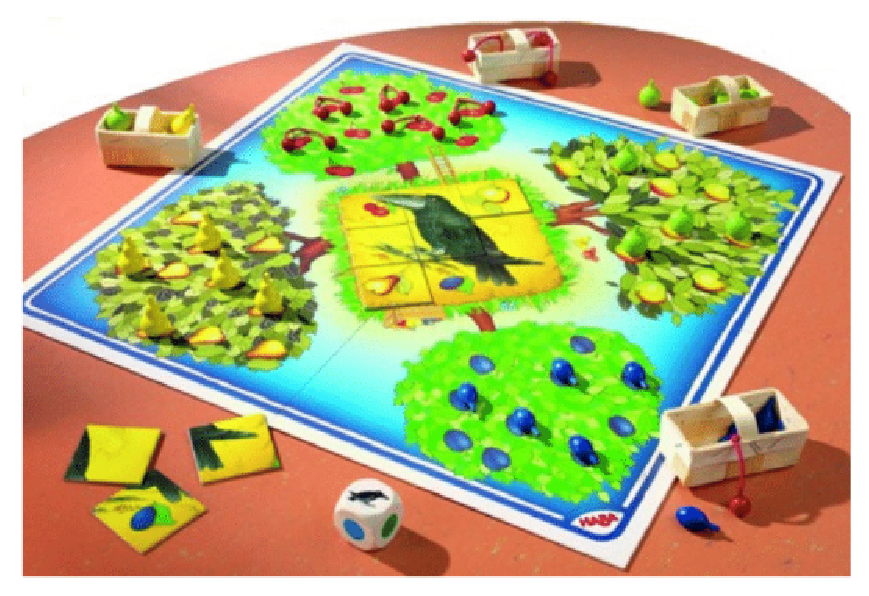
\includegraphics[scale=0.5]{img/verger.eps}
\end{center}

\subsubsection*{Règles du jeu}
Le but du jeu est de récupérer tous les fruits avant d'avoir reconstitué le puzzle du corbeau.

Un joueur lance le dé :
\begin{itemize}
\item Si le dé tombe sur un arbre, le joueur prend le fruit correspondant et le met dans son panier. S'il n'y a plus de fruit sur l'arbre, le joueur passe son tour.
\item Si le dé tombe sur le panier, le joueur prend 2 fruits de son choix.
\item Si le dé tombe sur le corbeau, il place une pièce du puzzle sur le corbeau.
\end{itemize}

\subsubsection*{Le gagnant}
Les joueurs gagnent tous ensemble s'ils ont réussi à cueillir tous les fruits de tous les arbres.
Les joueurs perdent ensemble si le puzzle du corbeau est reconstitué avant d'avoir cueilli tous les fruits.

\subsubsection*{Programmation}
Écrire un programme qui permet d'effectuer une partie et affiche le gagnant.


\newpage
\addtocounter{numexo}{1}
\subsection*{\Large Exercice \thenumexo }
Le jeu du loto se joue avec des grilles différentes composées de 15 numéros compris entre 1 et 90 (inclus). Au cours d'une partie, des numéros sont tirés au hasard. Le premier à avoir une grille complète est le gagnant du lot principal.

On donne un exemple de grille ci-dessous:

\begin{center}
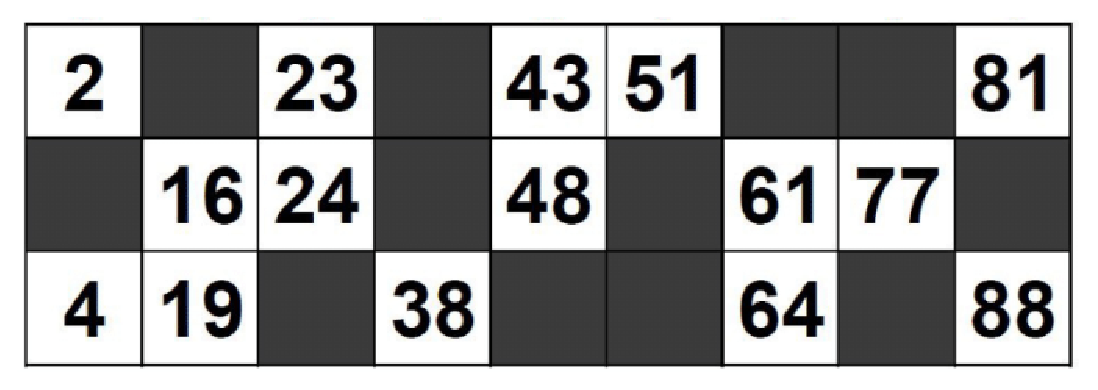
\includegraphics[scale=0.6]{img/loto.eps}
\end{center}

Écrire un programme produisant une carte de loto en respectant les contraintes suivantes :
\begin{itemize}
\item Une carte contient 9 colonnes et 3 lignes.
\item Il y a sur la carte 15 numéros différents choisis parmi les nombres de 1 à 90.
\item Chaque ligne contient 5 numéros (et donc 4 espaces vides).
\item Il y a toujours au moins un numéro par colonne.
\item Il peut y avoir 3 numéros dans une colonne, mais seulement dans la colonne 8.
\item La colonne 0 contient les numéros de 1 à 9.
\item La colonne 1 contient les numéros de 10 à 19.
\item La colonne 2 contient les numéros de 20 à 29.
\item ...
\item La colonne 8 contient les numéros de 80 à 90.
\end{itemize}


\end{document}

